\documentclass{beamer}
\usepackage[utf8]{inputenc}
\setbeamertemplate{itemize item}{\textbullet}	% Itemize dot symbol

\begin{document}

\title{Virtual Theremin}
\subtitle{UIE Project 2015}
\author{A. Alavi, P. Roos, A. Theler}
\date{\today} 

% N e w  F r a m e
\frame{\titlepage} 

% N e w  F r a m e
\frame{
    \frametitle{The Theremin}
    \begin{figure}[p]
        \centering
        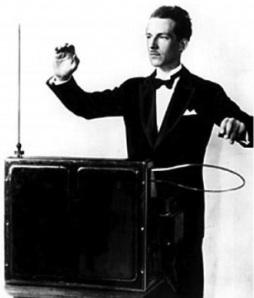
\includegraphics[height= 0.5\textwidth]{leontheremin.jpg}
        \caption{Léon Theremin playing his instrument}
    \end{figure}
}

% N e w  F r a m e
\frame{
    \frametitle{Virtual Theremin}
    Theremin controlled by position of hands. $\to$ Leap Motion Sensor to
    emulate a Theremin on your computer.
}

% N e w  F r a m e
\frame{
    \frametitle{Improvements}
    \itemize{
        \item Gestures for improved functionality and expressiveness of the
            instrument (Gestures like: close/open hand, pinching)
        \item Overcome instrument limitations
        \item Playing aid (frequency discretization)
    }
}

\end{document}
